\chapter{Konwolucyjna sieć Incepcja}
\label{chap:inception}

\section{Architektura sieci Incepcja}

\subsection{Wstęp}
Siec Incepcja (\textit{ang. Inception Network}) została zaprezentowana w 2015 roku w publikacji \textit{ang. Going deeper with convolutions} \cite{inceptionpaper}. 
Nazwa sieci (wraz z tytułem publikacji) nawiązuje do popularnego w tamtym czasie internetowego mema z Leonardo DiCaprio. 
Incepcja wychodzi naprzeciw problemom z treningiem bardzo głębokich sieci neuronowych. Jednym z nich jest rosnący margines błędu wraz rosnącą liczbą warstw co przedstawia rysunek \ref{fig:deep-error}.

\begin{figure}[ht]
\centerline{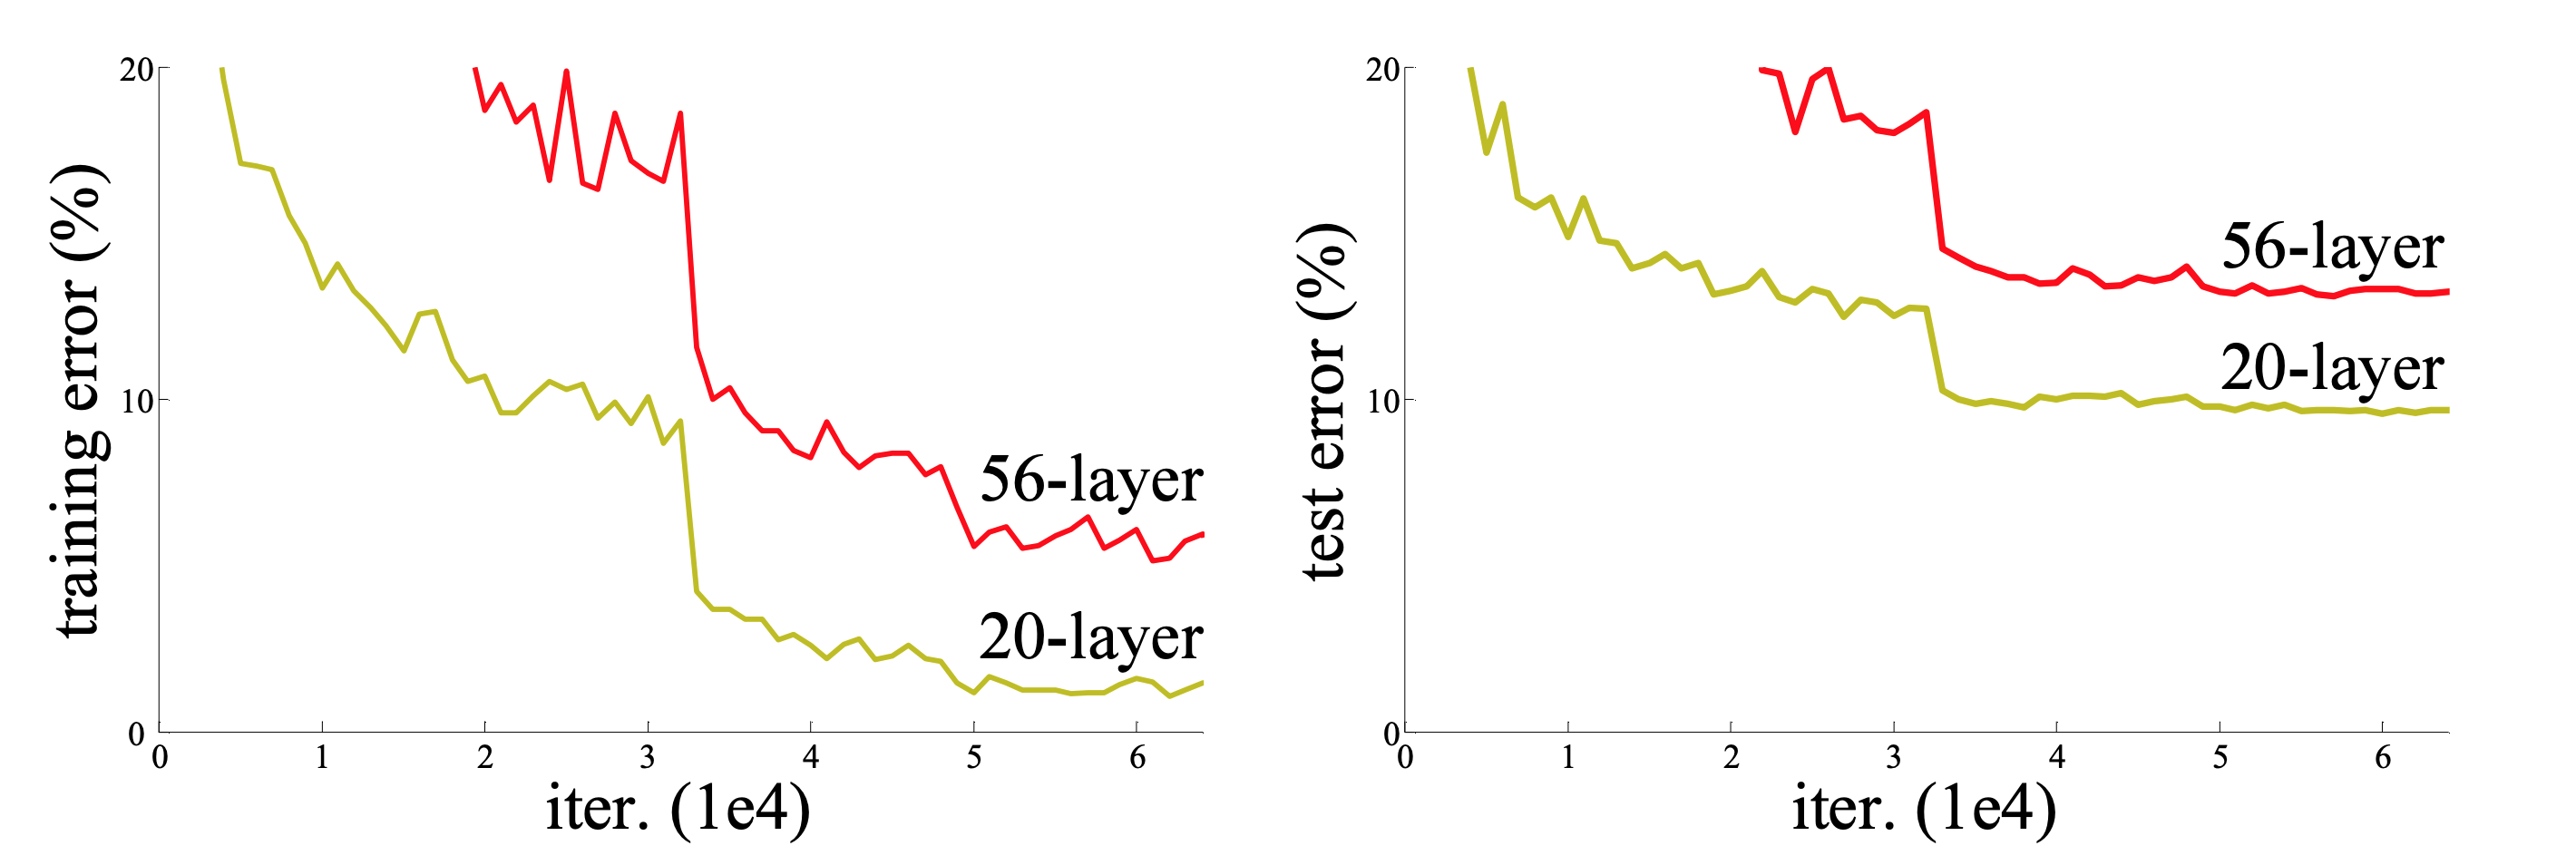
\includegraphics[scale=0.2]{resources/inception/deep-error.png}}
\caption{Błąd predykcji w stosunku do zastosowanej liczby iteracji treningowych przy uwzględnieniu liczby użytych warstw ukrytych dla standardowej architektury sieci neuronowej \cite{resnetpaper}.}
\label{fig:deep-error}
\end{figure}

Incepcja rozwiązuje ten problem rozbudowując się o dodatkowe operacje splotu w obrębie jednej warstwy-bloku (opisanego w podrozdziale \ref{subsection:inception-block}).
To wraz z zastosowaniem operacji splotu o wymiarach filtra \(1 \times 1\) (rysunek \ref{fig:dlawik}), sprawiło, że można było zbudować sieć o jeszcze większej liczbie warstw ukrytych, która jednocześnie zyskiwała na jakości predykcji.

\subsection{Blok sieci Incepcja}
\label{subsection:inception-block}
Główną cechą sieci typu Incepcja jest to, że jej architektura została rozbudowana o dodatkowe operacje splotu w obrębie jednej warstwy (rys. \ref{fig:inception-block}).
Mając do dyspozycji warstwę (lub \(N\) warstw) o wymiarach filtra \(W \times H\), stosujemy równocześnie splot o wymiarach filtra \(1 \times 1\), \(3 \times 3\), \(5 \times 5\) oraz warstwę \textit{MaxPool}. 
Wynik tych operacji konkatenowany jest i zapisywany jako warstwa wyjściowa. Wykonywane operacje splotu mają tak dobrane krok i dopełnienia, by wymiar \(W\) i \(H\) nie uległy zmianie. 
Taki dobór parametrów ma na celu łączenie jednego bloku sieci Incepcja bezpośrednio w drugi podobnie jak ma to miejsce w przypadku warstw sieci VGG. 
Podobnie jak w przypadku VGG, w celu modyfikacji dwóch pierwszych wymiarów warstwy stosowane są warstwy \textit{MaxPool} bezpośrednio między blokami incepcji.

\begin{figure}[ht]
\centerline{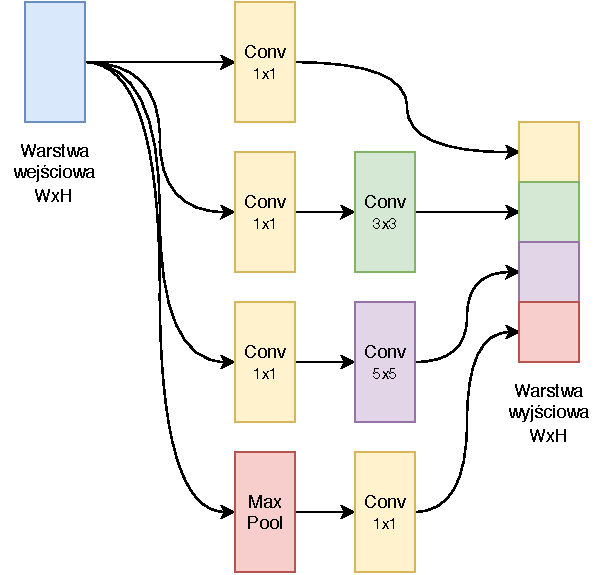
\includegraphics[scale=1]{resources/Inception_block.pdf}}
\caption{Schemat bloku z których składa się sieć Incepcja.}
\label{fig:inception-block}
\end{figure}

Operacje splotu o wymiarach \(1 \times 1\) są stosowane przed \(3 \times 3\) i \(5 \times 5\) w celu redukcji liczby warstw filtrów, co ma pozytywny wpływ na koszt obliczeniowy tej operacji (rys. \ref{fig:dlawik}).
Stosując \(F\) zestawów filtrów można dowolnie modyfikować trzeci wymiar uzyskanej warstwy. Dzięki temu, razem z \textit{MaxPool}, splot \(1 \times 1\) pozwala na dowolną modyfikację wymiarów uzyskiwanych konwolucji.

\begin{figure}[ht]
\centerline{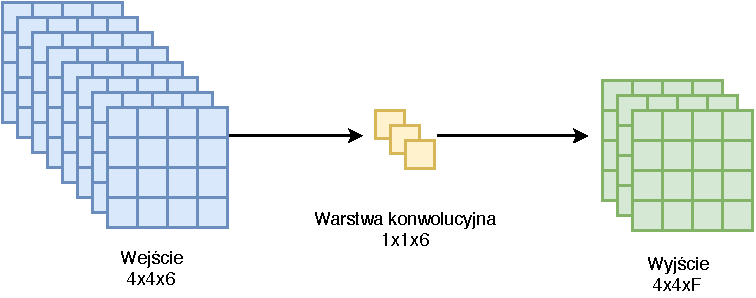
\includegraphics[scale=1]{resources/dlawik.pdf}}
\caption{Modyfikacja liczby warstw przy pomocy splotu \(1 \times 1\).}
\label{fig:dlawik}
\end{figure}

\subsection{Schemat sieci}

Zaprezentowany wariant sieci Incepcja, tak zwany GoogleLeNet (rys. \ref{fig:googleNet}) to 22 warstwowa sieć konwolucyjna. Oprócz widocznych dla Incepcji bloków, GoogleLeNet posiada 3 osobne warstwy
wyjściowe typu softmax. Każde z tych wyjść używane jest w czasie treningu do obliczania funkcji kosztu (ich koszt dodawany jest do całkowitego kosztu z wagą 0,3).
Autorzy twierdzą, że taka operacja ma właściwości regularyzujące wagi oraz pomaga z problemem zanikającego gradientu występującego przy tak głębokich sieciach neuronowych.
Te dodatkowe wyjścia nie biorą udziału w procesie testowania ani podczas pracy z danymi produkcyjnymi.
Między warstwami konwolucyjnymi a gęstopołączonymi znajduje się pierwszy w tej pracy przykład użycia \textit{AveragePooling}. Autorzy podają, że takie stosowanie \textit{AveragePooling} zwiększył dokładność najlepszych predykcji o około 0.6\%.
Z racji wielkości nie sposób zamieścić wszystkich informacji na temat sieci w postaci znanych do tej pory z tej pracy diagramów, dokładne informacje na temat użytych warstw zawiera tabela na rysunku \ref{fig:googleNettable}. Jest tam zaprezentowny również, obraz wejściowy dla algorytmu. Tym razem obraz nie był skalowany so przekłada się na duże zagszęszczenie wzoru.

\begin{figure}[ht]
\centerline{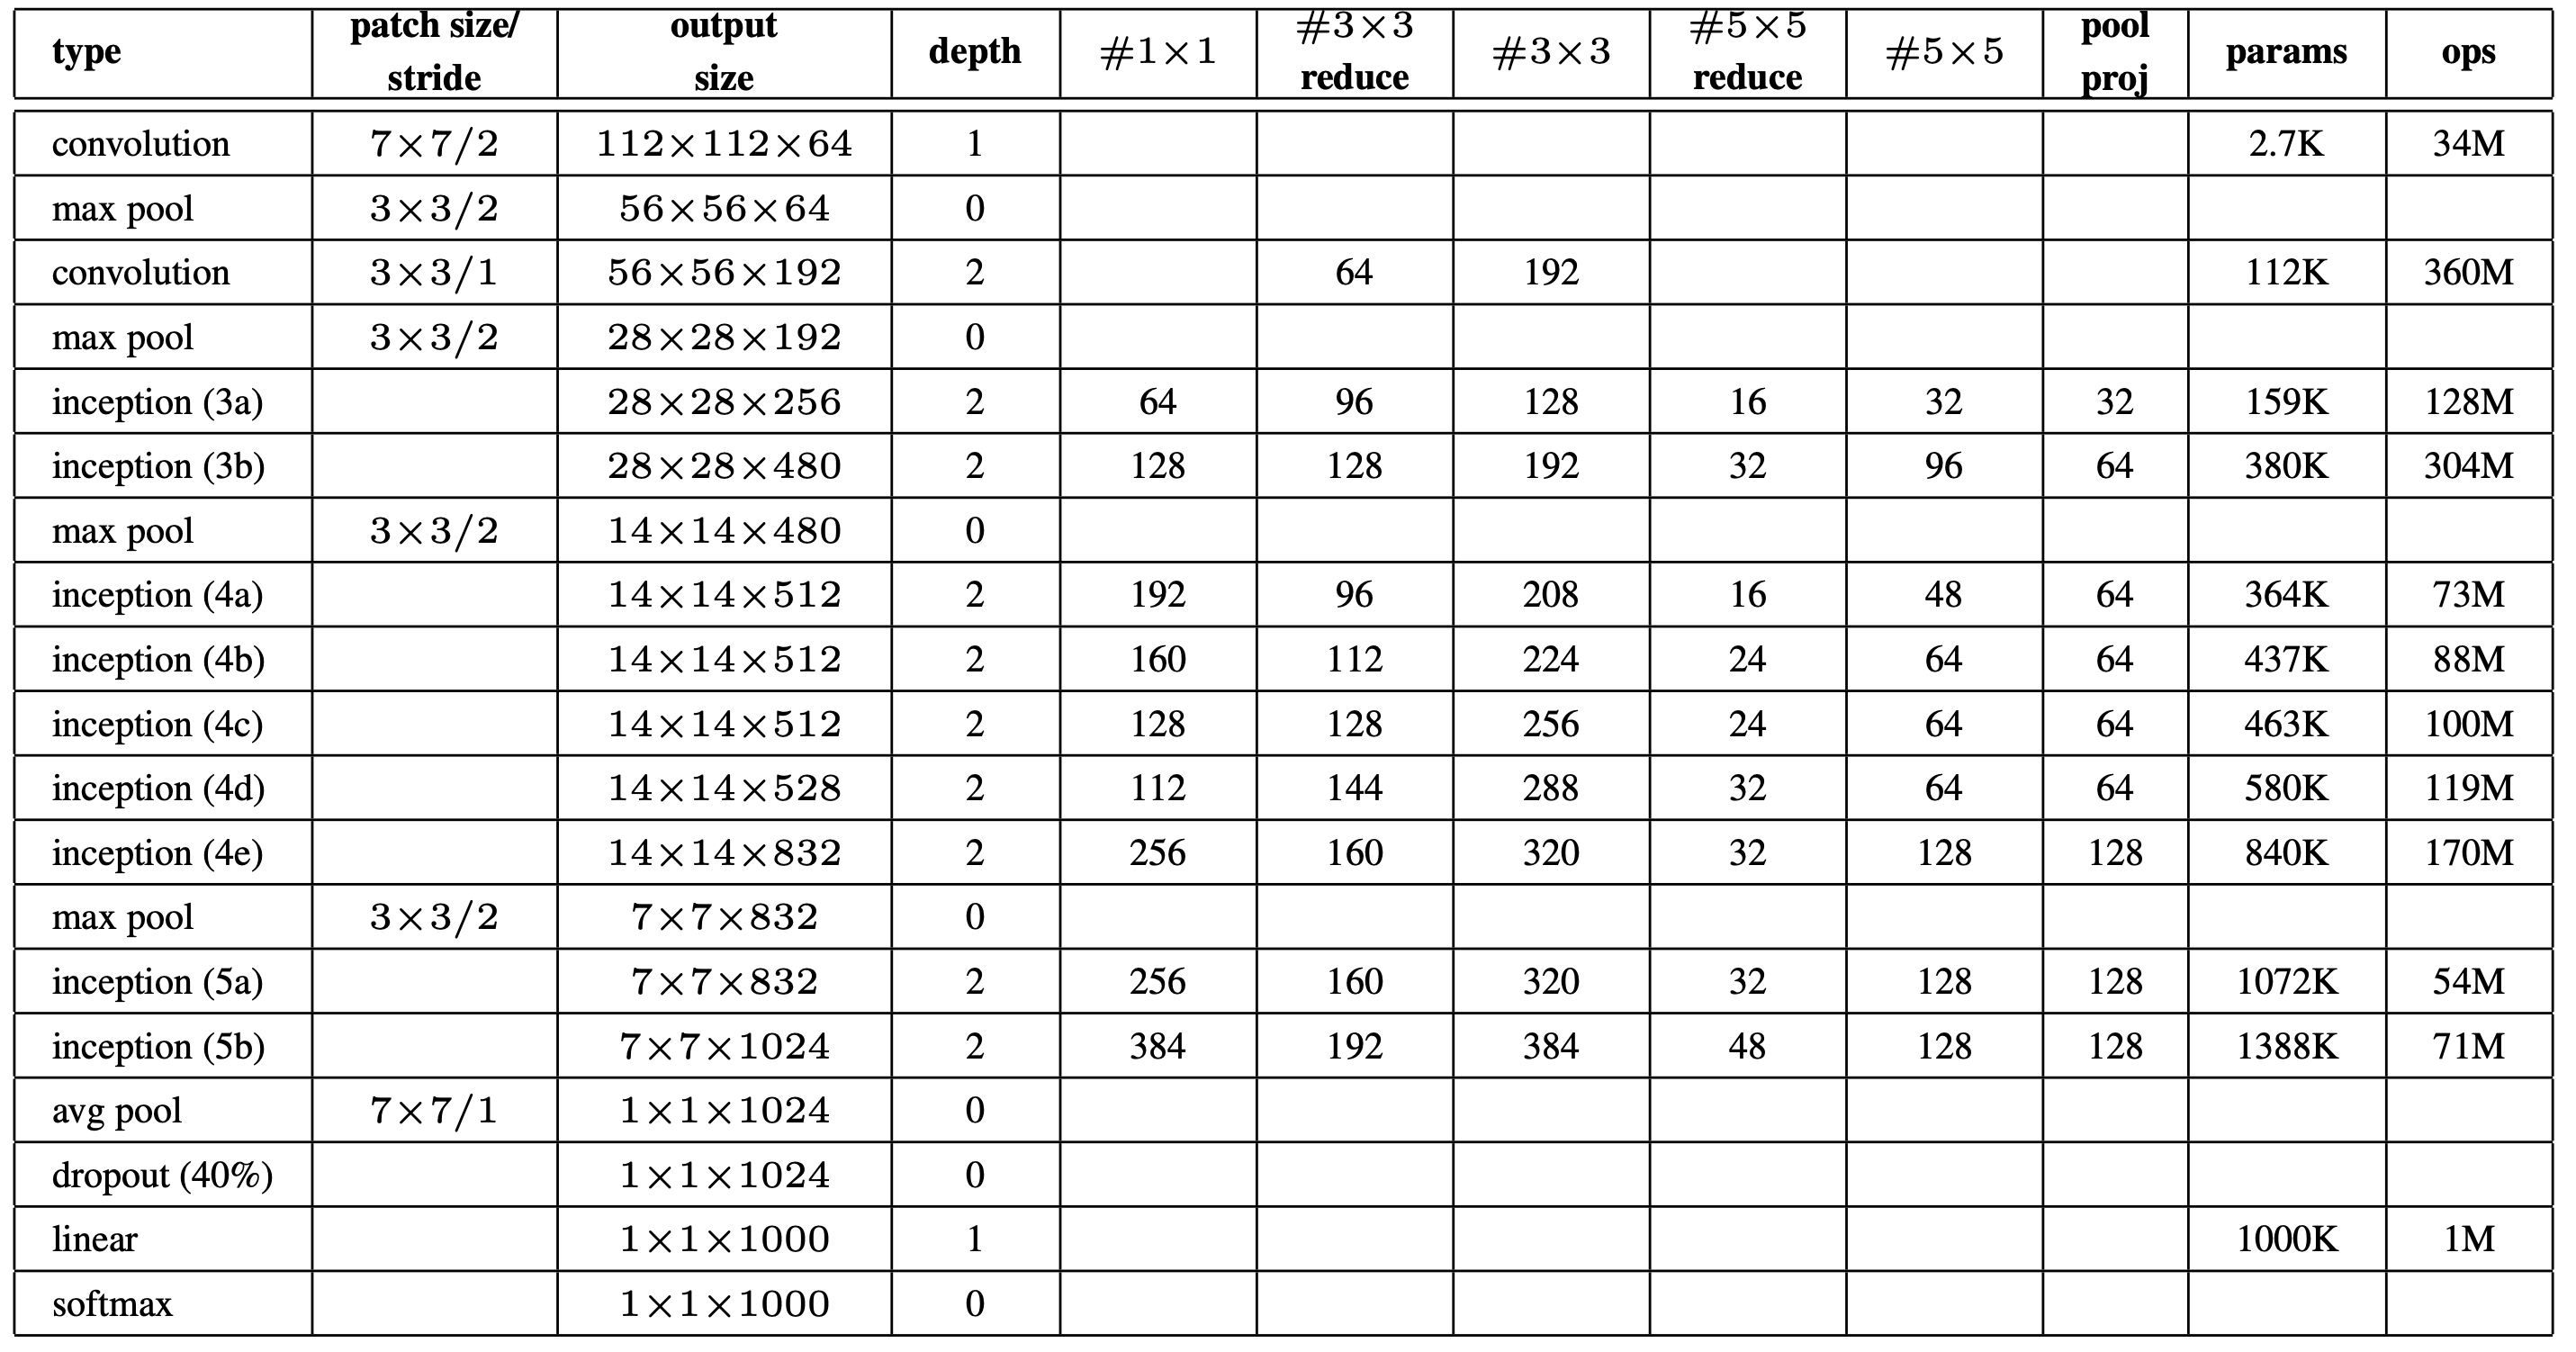
\includegraphics[scale=0.3]{resources/inception/googleNet-table.png}}
\caption{Szczegółowe dane na temat GoogleLeNet zaprezentowane w \textit{Going deeper with convolutions} \cite{inceptionpaper}.} 
\label{fig:googleNettable}
\end{figure}

\begin{figure}[ht]
\centerline{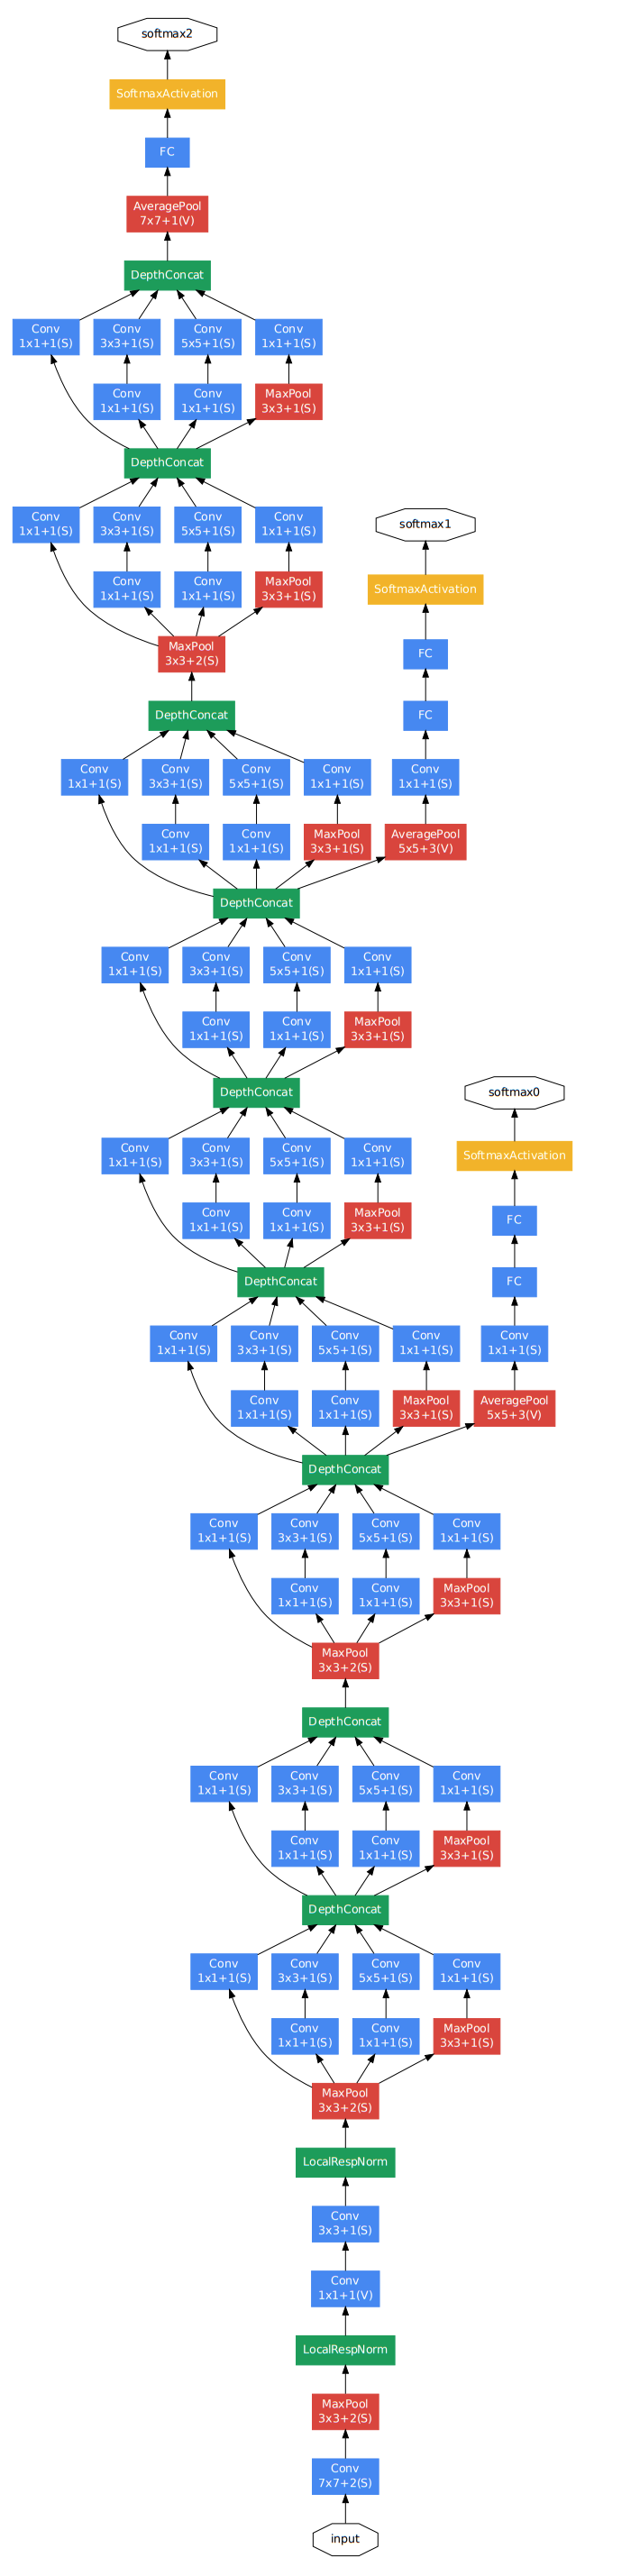
\includegraphics[scale=0.3]{resources/inception/googleNet.png}}
\caption{Schemat sieci GoogleLeNet zaprezentowany w \textit{Going deeper with convolutions} \cite{inceptionpaper}.} 
\label{fig:googleNet}
\end{figure}

\section{\textit{DeepDream} i wizualizacje warstw ukrytych GoogleLeNet}

\subsection{Opis i zasada działania}
\label{ddopis}
\textit{DeepDream} to  program komputerowy stworzony przez Aleksandra Mordvintseva. Został opublikowany  w 2015 roku i opisany w formie posta na blogu \cite{deepdream}.

Co do zasady działania, zarówno \textit{Deepdream}, jak i wizualizacje neuronów są modyfikacją programu zaprezentowanego w podrozdziale \ref{vgg-mean-activation}. Podobnie jak w wyżej wymienionym programie, używając wcześniej wytrenowanej sieci neuronowej modyfikujemy, obraz by zmaksymalizować aktywację neuronów danej sieci konwolucyjnej.

Poza oczywistą zamianą VGG na GoogleLeNet, \textit{DeepDream} stosuje znany już z podrozdziału
\ref{vgg-nst} sposób obliczania aktywacji kilku neuronów naraz, przy użyciu paramteru stopnia 
użycia danej warstwy \(\lambda\). Obliczając aktywację dla kilku warstw naraz uzyskuje się bogatsze w treść efekty wizualne. Podobnie jak w przypadku wizualizacji uzyskanych na VGG, w celu uzyskania obrazu, będę
modyfikować wcześniej spreparowany, wylosowany obraz-szum. W swoim poście oryginalny autor posłużył się kolorowym obrazem (RGB). Ciekawe efekty uzyskano również przy pomocy modyfikacji już istniejących zdjęć. Tak samo jak poprzednio, obraz jest wieloktronie skalowany podczas treningu, ale z racji swoich rozmiarów sieć GoogleLeNet jest w stanie uchwycić struktury nieuchwtyne dla VGG, co umożliwia generowanie 
nieco psychodelicznych obrazów.

\subsection{Wizualizacja warstw ukrytych modelu GoogleLeNet}
W przypadku wizualizacji samych warstw modelu GoogleLeNet zdecydowałem się na  
opublikowaną przez Google, opartą na \textit{tensorflow}, bibliotekę \textit{lucid} \cite{lucidrepo}. Jej głównym zastosowaniem jest wizualizacja neuronów, ale pozwala też m.in na \textit{neural style transfer}, nawet na obiektch 3D.

Podobnie jak w przypadku wizualizacji na VGG, nie będę trenował sieci Incepcja samodzielnie, ponieważ taki trening trwałby bardzo długo. Zamiast tego załaduję model przygotowany przez autorów biblioteki. Podobnie jak w przypadku VGG, model został wytrenowany na zbiorze \textit{ImageNet}.

\begin{lstlisting}[language=Python, caption={Wczytywanie modelu GoogleLeNet w \textit{lucid}.}, label={lst:load-model-lucid}, captionpos=b]
model = models.InceptionV1()
model.load_graphdef()
\end{lstlisting}

Po wczytaniu modelu (listing \ref{lst:load-model-lucid}) jedyne co pozostało, to wybrać warstwy, które chcemy aktywować i możemy generować wizualizacje.

\begin{lstlisting}[language=Python, caption={Generowanie wizualizacji neuronów przy użyciu \textit{lucid}.}, label={lst:visualise-lucid}, captionpos=b]
channel = lambda n: objectives.channel("mixed4a_pre_relu", n)
pf = lambda: param.image(256)
obj = channel(122) + channel(155)
_ = render.render_vis(model, param_f = pf, objective_f = obj)
\end{lstlisting}

Listing \ref{lst:visualise-lucid} jest przykładem implementacji wizualizacji aktywacji filtrów 122 i 155 warstwy \textit{mixed4a\_pre\_relu}.
Efekty skryptu można zobaczyć na rysunku \ref{fig:inc122i155}. Przykładowe wizualizacje innych filtrów i warstwy pokazuje rysunek \ref{fig:incOtherVis}.

Na załączonych wizualizacjach widać potencjał \textit{lucid} jako biblioteki. Uzyskane wyniki pokazują, w jaki sposób kolejne filtry oddziaływują na otrzymywany obraz -- opisują przez to interakcje między neuronami.

Liczba kombinacji między warstwami czy filtrami niestety nie pozwoli na zamieszczenie podobnego przeglądu aktywacji warstw, jaki został zamieszczony w przypadku sieci VGG. 
\begin{figure}[ht]
\centerline{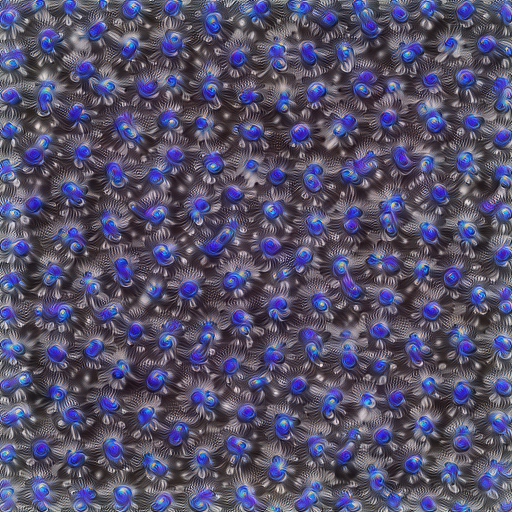
\includegraphics[scale=0.5]{resources/inception/mixed4a_pre_relu_122i155.png}}
\caption{Wizualizacja aktywacji filtrów 122 i 155 warstwy \textit{mixed4a\_pre\_relu}.}
\label{fig:inc122i155}
\end{figure}

\begin{figure}
\subfloat[Wizualizacja filtrów 122, 155 i 255 warstwy \textit{mixed4a\_pre\_relu}.]{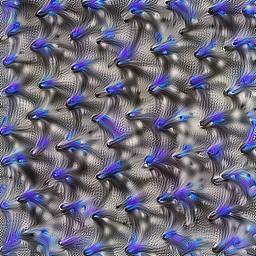
\includegraphics[width = 3in]{resources/inception/mixed4a_pre_relu_122i155i255.png}} 
~
\subfloat[Wizualizacja filtrów 122, 155, 255 i 455 warstwy \textit{mixed4a\_pre\_relu}.]{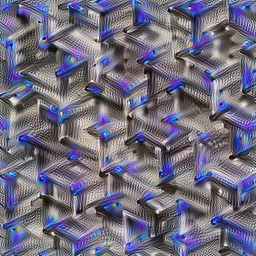
\includegraphics[width = 3in]{resources/inception/mixed4a_pre_relu_122i155i255i455.png}} 
\\
\subfloat[Wizualizacja filtra 1 warstwy \textit{mixed3a}.]{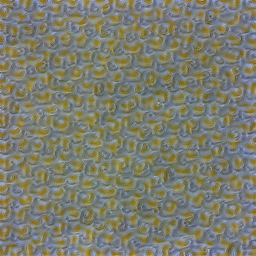
\includegraphics[width = 2in]{resources/inception/mixed3a_1.png}} 
~
\subfloat[Wizualizacja filtrów 1 i 102 warstwy \textit{mixed3a}.]{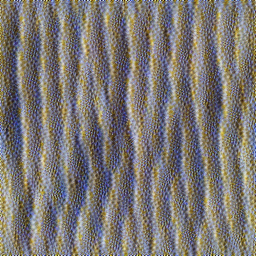
\includegraphics[width = 2in]{resources/inception/mixed3a_1i102.png}} 
~
\subfloat[Wizualizacja filtrów 1, 102 i 203 warstwy \textit{mixed3a}.]{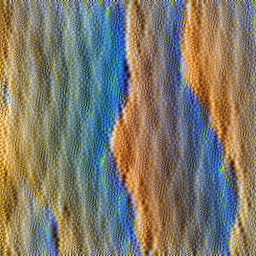
\includegraphics[width = 2in]{resources/inception/mixed3a_1i102i203.png}} 
\caption{Przykładowe wizualizacje neuronów sieci GoogleLeNet.}
\label{fig:incOtherVis}
\end{figure}

\subsection{Wizualizacje uzyskane przy pomocy \textit{DeepDream}}
Zgodnie z opisem z podrozdziału \ref{ddopis}, prezentowane wizualizacje zostały otrzymane poprzez modyfikację skryptu wizualizującego VGG. W procesie modyfikacji obrazu biorą 4 warstwy konwolucyjne (mixed od 2 do 4). Największy wpływ na funkcję kosztu mają 2 ostatnie warstwy. By uzyskać bardziej widoczny efekt, należy modyfikować oryginalny obraz przez większą liczbę iteracji, jest to jednak kosztowne obliczeniowo.

Uzyskane efekty zostały zaprezentowane na rysunku \ref{fig:deepdream}.

Charakterystyczny \textit{DeepDreamowy} wzór nabiera na wyrazistości wraz z kolejnymi iteracjami programu. Uzyskany efekt nie jest w stanie dać większego wglądu w sieci konwolucyjne i samą architekturę sieci Incpecja niż pokazane do tej pory wizualizacje, czy sposoby postępowania. Jednak to ten otrzymany efekt zdobył i utrzymuje pewien kultowy status, odgrywając niemałą rolę w popularyzacji sieci neuronowych i wiedzy o nich -- stąd chciałem by znalazł się też w mojej pracy.

\begin{figure}
\subfloat[Orginalny obraz, opuszczony kompleks narciarski obok Sarajewa. Autor zdjęcia: Kamil Mrzygłód.]{\includegraphics[width = 3in]{resources/inception/deepdream/1.png}} 
~
\subfloat[Wersja \textit{DeepDream} kompleksu narciarskiego.]{\includegraphics[width = 3in]{resources/inception/deepdream/skocznia4.png}} 
\\
\subfloat[Oryginalny obraz, most w miejscowości Mostar. Autor zdjęcia: Kamil Mrzygłód.]{\includegraphics[width = 3in]{resources/inception/deepdream/2.png}} 
~
\subfloat[Wersja \textit{DeepDream} mostu w Mostarze.]{\includegraphics[width = 3in]{resources/inception/deepdream/mostar.png}} 
\caption{Przykładowe wizualizacje neuronów sieci GoogleLeNet.}
\label{fig:deepdream}
\end{figure}

